 %%%%%%%%%%%%%%%%%%%%%%% file template.tex %%%%%%%%%%%%%%%%%%%%%%%%%
%
% This is a general template file for the LaTeX package SVJour3
% for Springer journals.          Springer Heidelberg 2010/09/16
%
% Copy it to a new file with a new name and use it as the basis
% for your article. Delete % signs as needed.
%
% This template includes a few options for different layouts and
% content for various journals. Please consult a previous issue of
% your journal as needed.
%
%%%%%%%%%%%%%%%%%%%%%%%%%%%%%%%%%%%%%%%%%%%%%%%%%%%%%%%%%%%%%%%%%%%
%
% First comes an example EPS file -- just ignore it and
% proceed on the \documentclass line
% your LaTeX will extract the file if required
%\begin{filecontents*}{example.eps}
%!PS-Adobe-3.0 EPSF-3.0
%%BoundingBox: 19 19 221 221
%%CreationDate: Mon Sep 29 1997
%%Creator: programmed by hand (JK)
%%EndComments

%\end{filecontents*}
%
\RequirePackage{fix-cm}
%
\documentclass{svjour3}                     % onecolumn (standard format)
%\documentclass[smallcondensed]{svjour3}     % onecolumn (ditto)
%\documentclass[smallextended]{svjour3}       % onecolumn (second format)
%\documentclass[twocolumn]{svjour3}          % twocolumn
%
\smartqed  % flush right qed marks, e.g. at end of proof
%
\usepackage{graphicx}
\usepackage{natbib}
\renewcommand{\figurename}{Fig.}
\newcommand{\reffig}[1]{Fig. \ref{#1}}
\usepackage{graphicx}
\usepackage{amsmath,amsfonts}
\usepackage{multirow,booktabs}
\usepackage{subfigure}
\usepackage{setspace}
\usepackage{lineno}
\usepackage{color}


%
% \usepackage{mathptmx}      % use Times fonts if available on your TeX system
%
% insert here the call for the packages your document requires
%\usepackage{latexsym}
% etc.
%
% please place your own definitions here and don't use \def but
% \newcommand{}{}
%
% Insert the name of "" with
\journalname{Plant and Soil}


%

\begin{document}
\title{Modeling the hydro-mechanical reinforcement of vegetation to the stability of a shallow slope based on the dynamic root growth
%\thanks{Grants or other notes
%about the article that should go on the front page should be
%placed here. General acknowledgments should be placed at the end of the article.}
}

%\titlerunning{Short form of title}        % if too long for running head

\author{Yang Yang$^1$
         %etc.
}

%\authorrunning{Short form of author list} % if too long for running head

\institute{ 
           $*$ Yang Yang  \at
              \email{smiba@qq.com}  
              \and
             1 College of Water Conservancy and Hydropower Engineering, Hohai University, Nanjing 210098, China \\
}

\date{Received: date / Accepted: date}
% The correct dates will be entered by the editor


\maketitle


\begin{abstract}





\keywords{Herb }
% \PACS{PACS code1 \and PACS code2 \and more}
% \subclass{MSC code1 \and MSC code2 \and more}
\end{abstract}

\section{Introduction}


\section{Methodology}

\subsection{The mechanical reinforcement model}





\subsection{Soil hydrological dynamic model}

The SWAP (Soil, Water, Atmosphere, and Plant) model has been applied widely to simulate soil water dynamics in the vegetated slope \citep{Romano2011Par}. In this study, we employed the Richards' equation to simulate the soils-vegetation-atmosphere interactions under unsaturated conditions; The modified Richards' equation can be written as follows:

\begin{equation}\frac{\partial \theta}{\partial t}=\frac{\partial}{\partial z}(k\frac{\partial h}{\partial z}) + S(z)\end{equation}
where $k$ is the unsaturated soil permeability at a given suction; $h$ is the hydraulic head; $x$, and $z$ are the coordinates in the horizontal and vertical directions, respectively; $\theta$ is the volumetric water content; $t$ is the time; $S$ is the source/sink term.



The soil water characteristic curve (SWCC) and hydraulic conductivity functions (HFC) are written according to the Van-Genuchten \cite{Genuchten1980A}
\begin{equation}\Theta=\frac{\theta-\theta_r}{\theta_s-\theta_r}=[\frac{1}{1+|\alpha h|^n}]^m\end{equation}
where $\Theta$ is the soil saturation; $\theta$ is the soil water content; $\theta_s$ is the saturated water content; $\theta_r$ is the residual water content; $n$ and $m$ are the shape parameters, if n $>$ 1, then $m = 1 - \frac{1}{n}$; $\alpha$ is a scale parameter.

\begin{equation}K(h) = K_s \Theta^{0.5}[1-(1-\Theta^{1/m})^m]^2\end{equation}
where $K(h)$ is the hydraulic conductivity at a given suction head $h$; $K_s$ is the saturated hydraulic conductivity. 

\subsection{Transpiration}
\begin{equation}ET_c=T_{pot}+E_{pot}=(K_{cb}+K_e)ET_0\end{equation}
where:

\subsection{Dynamic root growth model}
\subsubsection{Root penetration}
Root growth calculation is based on cumulative day-degrees, which is common for root models and has been shown in field trials to be applicable to both monocot and dicot crops \cite{PedersenModelling}. 

\begin{equation}DD = \left \{\begin{array}{c}0; \quad T_{min} \ge T_{air} \\
T_{air}-T_{min}\quad T_{min}; \le T_{air} < T_{max} \\
T_{max}-T_{min}\quad T_{air}; \ge T_{max}\end{array} \right.\end{equation}

The root penetration depth ($R_z$) is calculated as follows:
\begin{equation}R_z = \left \{\begin{array}{c}R_{z,min}; \quad \sum DD \le DD_{lag} \\
\sum ((DD-DD_{lag})k_{rz}+R_{z,min});\quad \sum DD>DD_{lag} \\
R_{z,min};\quad \sum(DD-DD_{lag})k_{rz}+R_{z,min}>R_{z,max}\end{array} \right.\end{equation}
where $DD$ is the Day-degress; $DD_{lag}$ is the lag phase for initiating root growth;
$R_{z,max}$ is the maximum rooting depth; $R_{z,min}$ is the rooting depth at sowing or planting; $T_{min}$ is minimum temperature for root growth; $T_{max}$ is the maximum temperature for root growth.

The root density distributions at different growth stages are quite similar, which indicate the feasibility of using a single normalized root density function for the whole growth season of each crop. A third-order polynomial equation was utilized to fit the pooled data of each crop as follows\cite{WuModeling}:
\begin{equation}L_{nrd}(z_r)=R_0+R_{1z_r}+R_{2z_r}^2+R_{3z_r}^3\end{equation}
where $R_i$ ($i$=0,1,2,3) are the polynomial coeffecients.


\subsubsection{Root density}

a simple normalized root density function
A third-order polynomial equation was utilized to fit the pooled data of each vegetation as follows:
\begin{equation}L_{nrd}(z_r) = R_0 + R_1z_r+R_2z_r^2+R_3z_r^3\end{equation}
where $R_i (i=0,1,2,3) $ are the polynomial coefficients.

\subsection{Infinite slope model}

For many rainfall-induced landslides, the failure surfaces are often shallow and parallel to the slope surface. The infinite slope model serves as an excellent illustration for slope stability analysis \citep{lu2013hill,Cho2002Eva}.
\cite{Lu2008Infinite} present a generalized framework for the stability of infinite slopes under steady unsaturated seepage conditions. This framework allows the water table to be located at any depth below the ground surface and variation of soil suction and moisture content above the water table under steady infiltration conditions. The schematic diagram of infinite slope is shown in \reffig{fig:sm}. The factor of safety ($F_s$) of a slope is evaluated as fellows:
\begin{equation}F=\frac{c_s+(\gamma z cos^2 \beta - \sigma^s) tan \phi^{'} }{\gamma z sin \beta cos \beta} \end{equation}
where $c_s$ is the soil effective cohesion; $\gamma$ is the soil specific weight of soil; $z$ is the depth of soil; $\beta$ is the slope angle; $\sigma^{s}$ is the suction stress characteristic curve; $\phi$ is the effective soil friction angle.

The suction stress can be expressed in terms of normalized volumetric water content or degree of saturation as \citep{Lu2008Infinite}:
\begin{equation}\sigma^s = -\frac{\theta-\theta_r}{\theta_s-\theta_r}(u_a-u_w)\end{equation}
where $\theta$ is the volumetric water content, $\theta_r$ is the residual volumetric water content; $\theta_s$ is the saturated volumetric water content; $u_a$ is the pore air pressure; $u_s$ is the pore water pressure.



For vegetated slope, the mechanical reinforcement provided by roots is quantified by means of a root cohesion term $c_r$ \citep{Pollen2007Temporal,Arnone2016Modeling}, so that the total cohesion of root-soil $c_{tot} = c_r+c_s$ and the factor of safety becomes
\begin{equation}F=\frac{c_r+c_s+(\gamma z cos^2 \beta - \sigma^s) tan \phi^{'} }{\gamma z sin \beta cos \beta} \end{equation}
which, after rearranging and applying trigonometric identities, becomes:
\begin{equation}F_s=\underbrace{\frac{tan\phi^{'}}{tan\beta}}_{1}+\underbrace{\frac{2c_s}{\gamma z sin2\beta}}_{2}+\underbrace{\frac{2c_r}{\gamma z sin2\beta}}_{3} 
-\underbrace{\frac{\sigma^s(tan\beta+cot\beta)tan\phi^{}}{\gamma z}}_{4}\label{1}\end{equation}
In the Eq.(\ref{1}), terms 1 and 2 are, respectively, the slope stability contribution due to the internal frictional $\phi^{'}$ and the soil cohesion $c_s$. Terms 3 and 4 are, respectively, the slope stability contribution due to the root cohesion $c_r$ and the suction stress.

\begin{figure*}
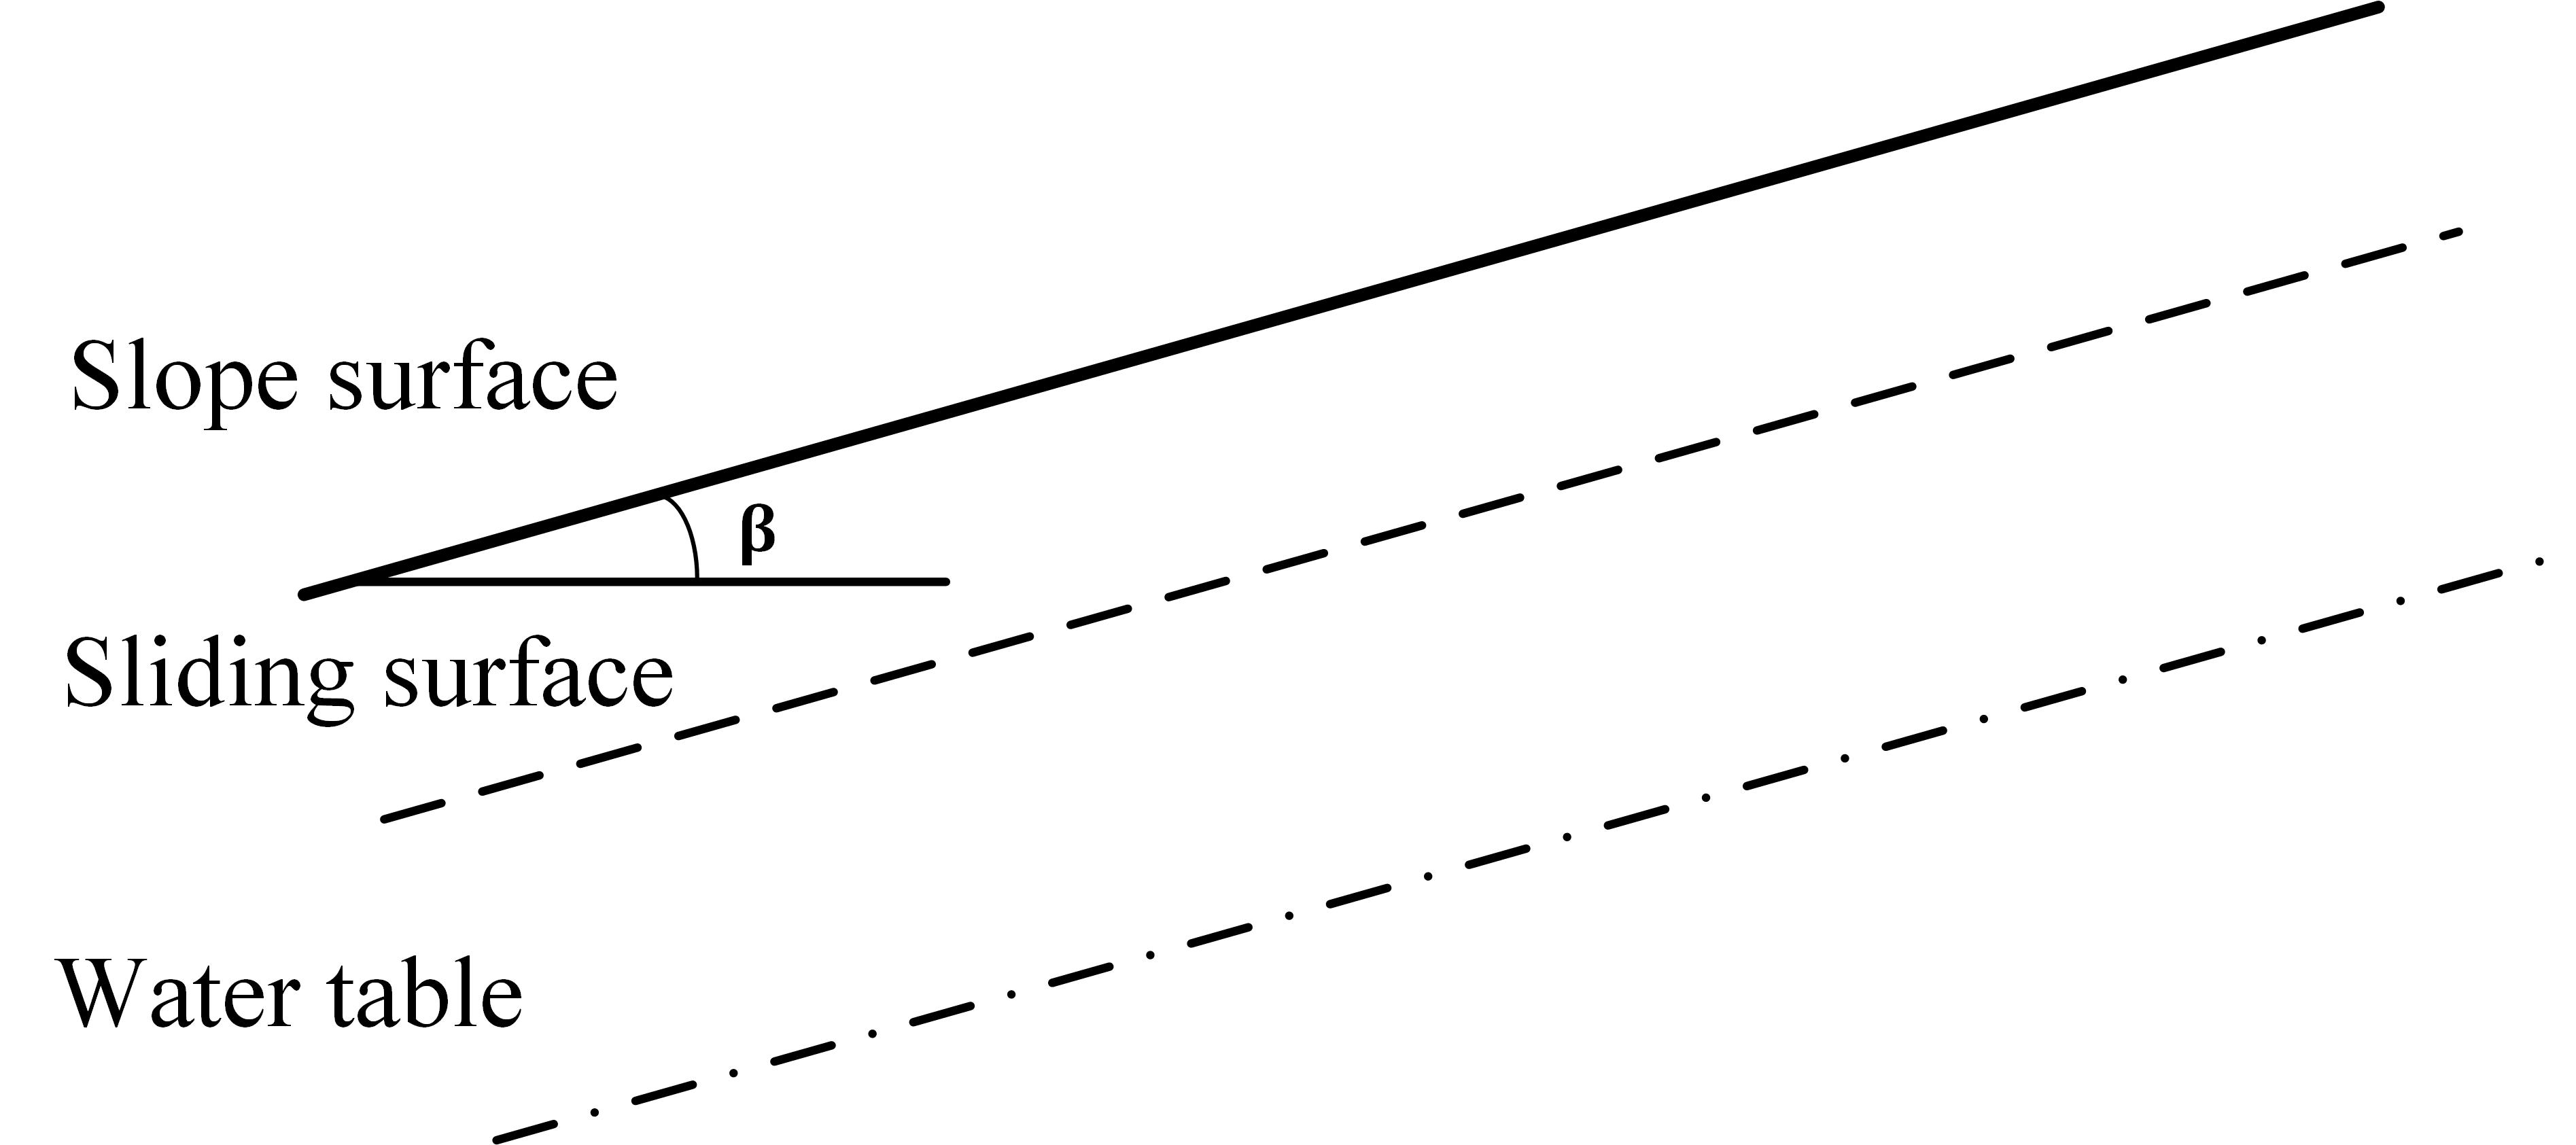
\includegraphics[width=1.0\textwidth]{slopemodel.jpg}
\caption{Schematic diagram of infinite slope}
\end{figure*} 
\label{fig:sm}





\section{Result}


\subsection{Effects of root system on the slope stability}


\subsection{Effects of slope geometry on the slope stability}


\section{Discussion}


\section{Conclusion}



\section{Acknowledgment}




% BibTeX users please use one of
\bibliographystyle{spbasic}      % basic style, author-year citations
%\bibliographystyle{spmpsci}      % mathematics and physical sciences
%\bibliographystyle{spphys}       % APS-like style for physics
%\bibliographystyle{model4-names}
\bibliography{mybibfile}   % name your BibTeX data base

% Non-BibTeX users please use
%\begin{thebibliography}{}
%
% and use \bibitem to create references. Consult the Instructions
% for authors for reference list style.
%

% etc

\end{document}

% end of file template.tex